
\providecommand{\myrootdir}{..}
\documentclass[\myrootdir/main.tex]{subfiles}

\begin{document}

\chapter{LogChunks Data Set}
\label{sec:data-set}
\includegraphics[page=5, width=\textwidth, trim={0.5cm 0.5cm 0.5cm 0.5cm}, clip]{img/flow-of-research.pdf}
This chapter describes the creation of the \emph{LogChunks} data set that we use in our empirical comparison of chunk retrieval techniques.
\emph{LogChunks} is a collection of 797 Travis CI build logs from 80 GitHub repositories spread over 29 programming languages.
For each build log we manually labeled which substring describes why the build failed.
The data set also provides keywords a developer would use to search for the labeled log chunk and categorizes the log chunks according to their format within the log.

We start this chapter by explaining why we created \emph{LogChunks} and how it enables us to compare the chunk retrieval techniques PBE, CTS and KWS\@.
Then, we introduces related data sets and show how \emph{LogChunks} differs.
The chapter describes the data schema of \emph{LogChunks} and our log collection process.
Further, it presents the labeling process and how we validated the labeled data, including a survey of the original developers of the projects represented in \emph{LogChunks}.
%In the first validation study, we compared the labeled data points with those of a second labeler on a sample of the build logs.
%For the second validation study, we sent out mails to the original project developers to determine whether the substring we labeled really describes the reason the build failed.

\section{Motivation}
\todo{In/output examples (I/O examples) are used to configure two of the information retrieval techniques we are evaluating for this thesis, PROSE regular expression program synthesis by example and text similarity.
One example set always contains build log in/output examples from the same software repository or project and for one specific build log information. They are all from one repository because we investigate information retrieval techniques which are always configured to the scope of one particular software repository or project.
Our intuition was that the ability of PROSE to be able to successfully learn a regex program depended on the structural uniformity of the provided in/output examples.
The regular expressions need a consistent pattern in the build log string at the borders or around the textual representation of a build log information to match on for the retrieval.
To be able to quantify this intuition in our evaluation we assigned \emph{structural categories} to each of the examples within an example set.}

\section{Related Data Sets}
\label{sec:related-data-sets}
This section presents existing data sets of CI build logs and why \emph{LogChunks} is unique among them.

\subsection{TravisTorrent}
The \emph{TravisTorrent} data set~\cite{beller2017travistorrent} collects a broad range of metadata about builds on Travis CI\@.
It combines data accessible through the public Travis CI API~\cite{travisci2019apidoc}, related data from GHTorrent~\cite{gousios2013ghtorrent}, the corresponding git repository and data obtained through analysis of the build logs.
The data obtained through build logs contains the names of failing test cases, similar to the reason the build failed in \emph{LogChunks}.
However, these values are obtained through a manually developed parser, which only supports specific Ruby test runners and Java Maven or JUnit logs.
\emph{LogChunks} provides manually labeled data points on the description of the build failure reason for a much wider selection of programming languages.

\subsection{Travis CI Build Log Data Set}
Loriot et al.~\cite{loriot2019dataset, loriot2019styler} collected a large amount of Travis CI build logs from 130 github repositories to analyze their use of the Checkstyle plugin.
They selected Maven repositories that included the Checkstyle plugin and also used Travis CI\@.
Their data set only provides the plain build logs, whereas \emph{LogChunks} additionally provides manually labeled data about the chunk describing why a build failed.

\section{Data Schema}
\label{sec:data-schema}
This section describes the file structure and the data schema of \emph{LogChunks}.
We give a detailed explanation for the manually labeled data.

\emph{LogChunks} has two top level folders, \texttt{logs} and \texttt{build-failure-reason}.
Each contains folders representing the main languages of the repositories in \emph{LogChunks}.

The logs are organized in folders for each repository, identified through the repository slug: \texttt{\textless repository\_owner\textgreater @\textless repository\_name\textgreater }.
Within each repository folder the logs are separated according to build status.
Currently \emph{LogChunks} only contains logs from \texttt{failed} builds.
The build status folder contains the full logs in files named with the ID of the Travis CI build that produced the log.

The folder \texttt{build-failure-reason} contains the manually labeled data of \emph{LogChunks}.
The data set provides an XML file for each repository \texttt{\textless repository\_owner\textgreater @\textless repository\_name\textgreater .xml}) categorized according to the main language of the repository.
The schema of these XML files is presented in Listing \ref{lst:examples}.

\lstset{
  language=XML,
  morekeywords={Examples, Example, Log, Keywords, Category, Chunk},
  postbreak=\mbox{\textcolor{blue}{$\hookrightarrow$}\space},
	frame=single
}
\begin{lstlisting}[caption={Example XML file from \emph{LogChunks}}, label=lst:examples, breaklines=true]
<Examples>
  <Log>C/php@php-src/failed/529279089.log</Log>
    <Keywords>ERROR, FAIL, DIFF</Keywords>
    <Category>0</Category>
    <Chunk>001+ ** ERROR: process timed out **

001- OK.
========DONE========
FAIL Bug #60120 (proc_open hangs when data in stdin/out/err is getting larger or equal to 2048) [ext/standard/tests/file/bug60120.phpt]</Chunk>
  </Example>
  ...
</Examples>
\end{lstlisting}

For each repository, \emph{LogChunks} gives about 10 \texttt{Examples}.
Each \texttt{Example} consists of:
\begin{itemize}
	\item \texttt{Log:} the relative path to the input build log.
	\item \texttt{Chunk:} the targeted information chunk. We are targeting the substring of the log that describes why the build failed.
	\item \texttt{Keywords:} keywords a developer would use to search for the log chunk.
	\item \texttt{Category:} a categorization of the structural representation of the log chunk within the build log.
				The category is relative to the other examples for the same repository.
\end{itemize}
Following, this section defines in more detail the labeled log chunk, search keywords and structural categories.

\paragraph{Chunk Describing Why The Build Failed}
The \texttt{Chunk} is the substring of the build logs that describes why the build failed.
This could be the failing test case, the description of a failed linter rule or a compiler error.
The \texttt{Chunk} is one continuous string cut from the build log.
If there are multiple errors leading for the build to fail, the substring contains the first appearing continuous error descriptions.
\emph{Continuous} means that no lines reporting of normal build behavior are interrupting the error descriptions.
Wherever possible, it does \emph{not} include the log statements describing \emph{that} the build failed, but the description of \emph{why} it failed.
For a few logs we were unable to define the section detailing why the build failed, e.g.\ because this information was logged in another log file.
In these instances the \texttt{Chunk} contains the lines describing that the build failed.

\paragraph{Keywords}
The \texttt{Keywords} contain a list of one to three keywords appearing within the \texttt{Chunk} or in the area around it in the build log.
We aim to select keywords a developer would use to search for the \texttt{Chunk} when inspecting the build log.

\paragraph{Category}
For each repository, we assign \emph{structural categories} to the examples.
The structural category compares how the \texttt{Chunk}s are represented within the build logs.
Build tools highlight their error messages with markings, e.g.\ starting each line with ``\texttt{ERROR}'', surrounding lines filled with special characters or additional empty log lines.
Two examples fall into the same structural categories if they are surrounded by similar markings.
For most cases, two \texttt{Chunk} examples that fall into one category are outputted either within the same build phase or by the same build tool.
For each repository, the structural categories are represented as integers, starting at 0 and increased with the next appearing category in chronological build order.

\section{Log Collection}
We describe how we select the repositories, builds and logs for \emph{LogChunks}.
To collect the build logs we built the  \texttt{GHTorrentParser}, \texttt{LogCollector} and \texttt{TravisRequester} using Ruby.

\paragraph{Repository Sampling}
First, we determine a set of repositories to query logs from.
Our \texttt{GHTorrentParser} queries the \emph{GHTorrent}~\cite{gousios2013ghtorrent} data set for the most popular languages on GitHub~\cite{github2019website}.
It then retrieves the most popular repositories for a given language.
We define \emph{Popularity} as the number of watches.
The \texttt{TravisRequester}, our tool querying the Travis API~\cite{travisci2019apidoc}, can then check for a given repository whether it uses Travis CI\@.

For \emph{LogChunks} we queried GHTorrent from 01/04/2018 for the three most popular repositories of each of the 30 most popular languages.

\paragraph{Build Sampling}
The \texttt{LogCollector} uses the \texttt{TravisRequester} to obtain the newest builds for a given repository.
It uses a stratified sampling approach: \texttt{TravisRequester} saves the obtained builds in buckets according to their status.
We encountered the following statuses during our data collection: created, started, cancelled, passed, errored and failed.
The user of \texttt{TravisRequester} configures how many builds should be checked and how many builds per status should be saved.

To sample the builds for \emph{LogChunks} we let \texttt{TravisRequester} check up to a 1000 builds per repository and keep ten for each status.
We discard all statuses except \emph{failed}~\cite{travis2009buildstatus}.
A Travis CI build is marked as \emph{failed} when it faults in the \texttt{script} section of the build configuration defined by the user.

\paragraph{Log Sampling}
For each build the \texttt{TravisRequester} then selects a log to download.
Travis CI attributes logs to \emph{jobs}.
A single build can consist of multiple jobs, e.g.\ building the same code version and executing tests in various different testing environments.
A failed build can have successful job executions, as just one failed job leads to the whole build being marked as failed.
\texttt{TravisRequester} queries each build for the first job, which has the same state.
For the selected jobs, the tool queries the Travis API V3 over HTTPS to obtains the corresponding build log.

We manually inspected the collected build logs and had to discard logs from three repositories.
One had only a single failed build, two others had empty build logs on Travis CI\@.
In total we collected 797 logs from 80 repositories.

\section{Labeling Process}
\label{sec:labeling-process}
After collecting a wide range of Travis CI build logs we manually labeled which text chunk describes why the build failed.
Following that, we assigned search keywords and structural categories to each log chunk.

\paragraph{Chunk Describing Why The Build Failed}
For each repository, the labeler skimmed through the build logs and tried to identify the first occurrence of a description why the build failed.
They copied out the first continuous description as the \texttt{Chunk}.
They preserved whitespace and special characters, as they might be crucial to detect the targeted substring.
To support exact learning of regular expressions identifying the labeled substrings the labeler aimed to start and end the labeled substring at consistent locations around the fault description.

\paragraph{Keywords}
We presented the \texttt{Chunk} and ten lines above and below to the labeler.
Their task was to note down three strings they would put into a document search function to find this failure description.
The string should appear in or around the \texttt{Chunk} substring and is case-sensitive.
There are no special limitations on the string itself, especially spaces are also allowed.

\paragraph{Category}
To label the \emph{structural categories} we again presented the \texttt{Chunk} and the surrounding context to the labeler for all logs from a repository.
We asked them to assign numerical categories according to whether the \texttt{Chunk} had the same structural representation, i.e.\ the same surrounding or identifying characters.
The labeler should start the categories with 0 and increase as new ones appear.
For reproducibility we presented the logs in chronological build order.

\section{Validation}
We validate our collected data points in two different ways.
A different labeler performed a second pass of labeling the build failure reason, keywords and structural categories on a subset of the data.
In addition, we sent out a survey to the developers, whose commits triggered the builds within our data set.
We asked them whether our retrieval of the log part describing the reason the build failed was correct.
This sections describes these two validation studies.

\subsection{Inter-Rater Reliability Study}
To evaluate the validity of our labeled data points we perform a second labeling of a sample of the data in \emph{LogChunks}.

\paragraph{Method}
The second labeler processed 30 random generated logs for each data point in \emph{LogChunks}.
We followed the same labeling process as described in Section~\ref{sec:labeling-process}.
For the build failure reason and the keywords, we presented 30 randomly sampled build logs from distinct repositories in \emph{LogChunks}.
The labeled structural categories are relative to the other logs from the same repository.
Therefore, we randomly sampled 3 repositories and presented all 10 examples within them to the second labeler.

\paragraph{Results}
For the first labeled data point, namely the substring describing why the build failed, the two labelers exactly agreed in six cases.
In 15 cases the second labeler selected more lines than the first one, in five there was partial overlap and in 4 they completely disagreed.

Regarding the keywords the two labelers completely agreed in nine cases and completely disagreed in two cases.
In nine cases there was partial overlap in the keywords of the two labelers, in two the first labeler selected additional keywords compared to the second, while the second labeler proposed additional keywords in seven cases.

When classifying the labeled substrings into structural categories, the two labelers agreed in 26 cases and disagreed in four cases.

\paragraph{Discussion}
The results of this validation study show that there is overlap in the data from both labelers, however also a high variation.
We believe that the main cause for this is that our explanations to the second labeler were not extensive enough.
There were implicit, inconsistent assumptions both labelers created during their work.
In the following we describe these assumptions from both labelers for each data point and the implications on our description of the data classes.

For the first data class, the reason the build failed, it was ambiguous whether the labeled substring should contain the information \emph{that} the build failed.
This concerns statements like ``\texttt{The build exited with 1}''.
One labeler included such statements, while the other one only focussed on the log parts describing \emph{why} the build failed, e.g.\ the name of the failing test case.

While labeling the keywords a developer would use to search for the log part describing why the build failed, the one labeler allowed arbitrary strings appearing around the presented log part.
In contrast to that, the other labeler focussed on actual \emph{words}, delimited by spaces or special characters.
One labeler ignored capitalization, while the other one selected case-sensitive keywords.
A third difference was that the first labeler was presented with all substrings from a repository, yielding more general keywords than the second labeler.

For the structural categories this validation study showed a high overlap.
In our instructions to the second labeler we did not emphasize the \emph{structural} aspect enough.
They sorted into categories along \emph{why} the build failed, putting failing tests from different test runners into the same category even though the failing tests were presented differently in the log.

Our main learning from this study is that adequately communicating all decisions and assumptions on how data is labeled is important and difficult.
We reviewed the misunderstandings and incorporated more thorough descriptions of our data classes in Section~\ref{sec:data-schema}.

\begin{figure}[h]
	\centering
	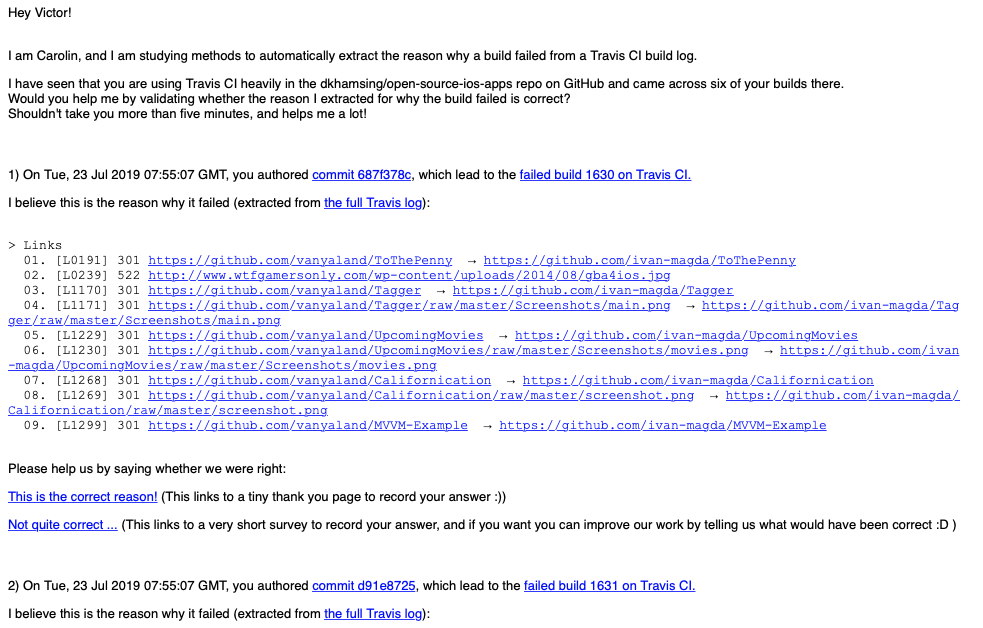
\includegraphics[width=\textwidth, clip]{img/dev-mail.png}
	\caption{An example of the mails we sent out to developers for validation of our labeled log part}
	\label{fig:dev-mail}
\end{figure}
\begin{figure}[h]
	\centering
	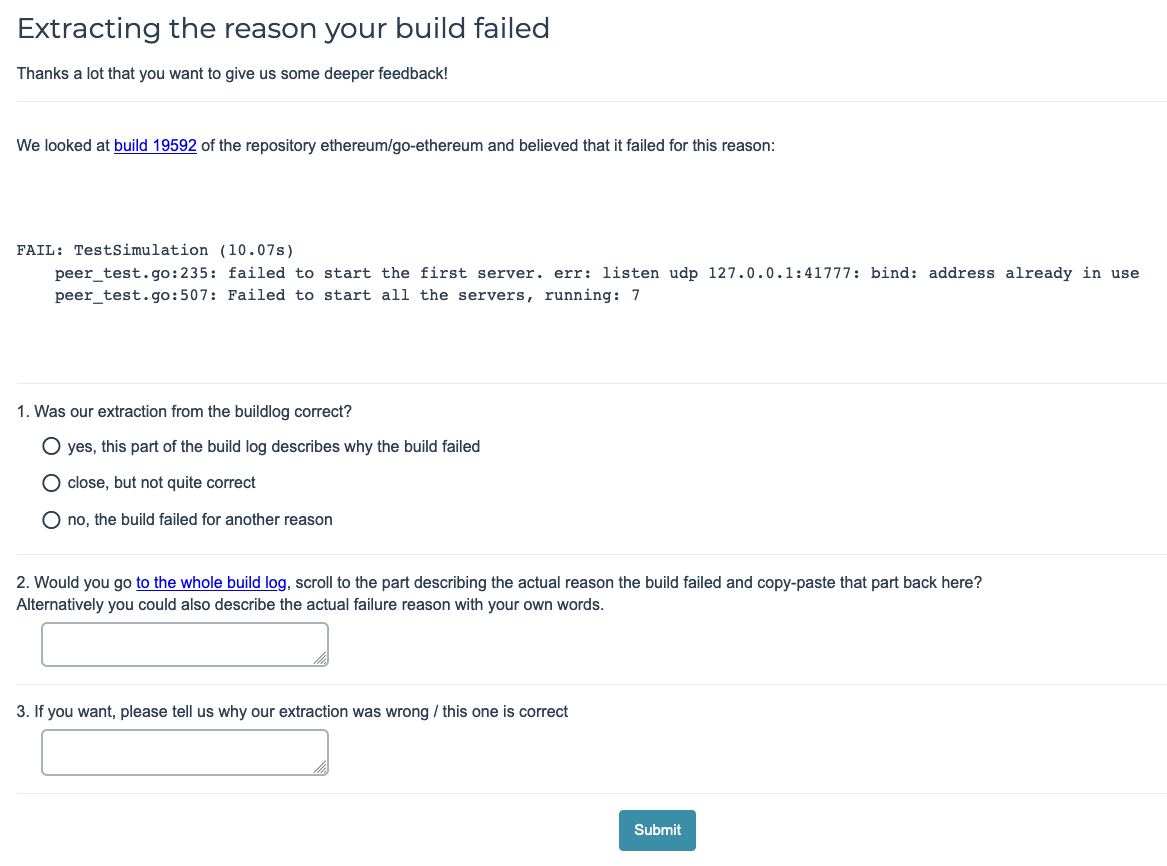
\includegraphics[width=\textwidth, clip]{img/dev-survey.png}
	\caption{Survey for the validation with developers}
	\label{fig:dev-survey}
\end{figure}

\subsection{Developer Survey}
For \emph{LogChunks} we analyzed around 800 build logs from different repositories and tried to extract the part of the log which describes why the respective build failed.
As we are not involved in the development of any of the projects within our data set we could only rely on our previous experience with various build logs and systems.
We only took the logs into accont and did not check the related configurations, so it is well possible that we extracted parts that do describe errors but the respective step failing is ignored by the configuration and the build failed for another reason.

The person who probably knows best why a build failed is the one committing the changes which triggered the build.
If the build was e.g.\ part of a pull request then developer likely inspected the failed build and tried to fix the build so the pull request can be accepted.
We sent out mails to the original developers whose commits triggered the builds represented in \emph{LogChunks} and asked them whether the log chunk we labeled actually describes why the build failed.
This section describes out survey and discusses our results.

\paragraph{Method}
Using the Travis API, for every build log in the data set we looked up the corresponding build and the committer information.
We grouped all commits triggered by one developer and sent out a mail to each of them, asking whether the log part selected during our labeling was indeed describing the reason the build failed.
Figure~\ref{fig:dev-mail} shows one of the mails sent out.
The mail included links to the corresponding commits, build overview and log file.
We asked the receivers to fill out a short survey in case our extraction was not correct.
Look at Figure~\ref{fig:dev-survey} to get an impression of the survey.
In the survey we presented the selected log part and asked the developer to paste in the log part actually describing the failure reason or describe why we were wrong in their own words.
As some of the extractions we labeled are many lines long, we trimmed all down to 10 lines to keep the mail readable.

\begin{figure}[htbp]
	\centering
	\begin{minipage}{0.45\textwidth}
		\centering
		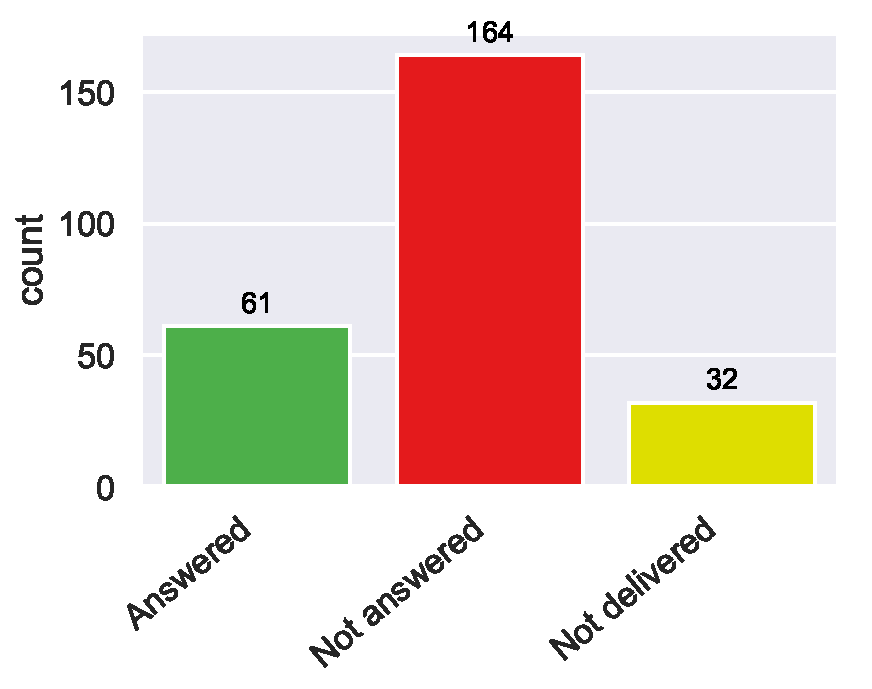
\includegraphics[width=\textwidth, clip]{img/dev-mails/answers-received-mails.pdf}
		\caption{Number of mails answered, unanswered and not delivered}
		\label{fig:mails-answers-received-mails}
	\end{minipage}\hfill
	\begin{minipage}{0.45\textwidth}
		\centering
		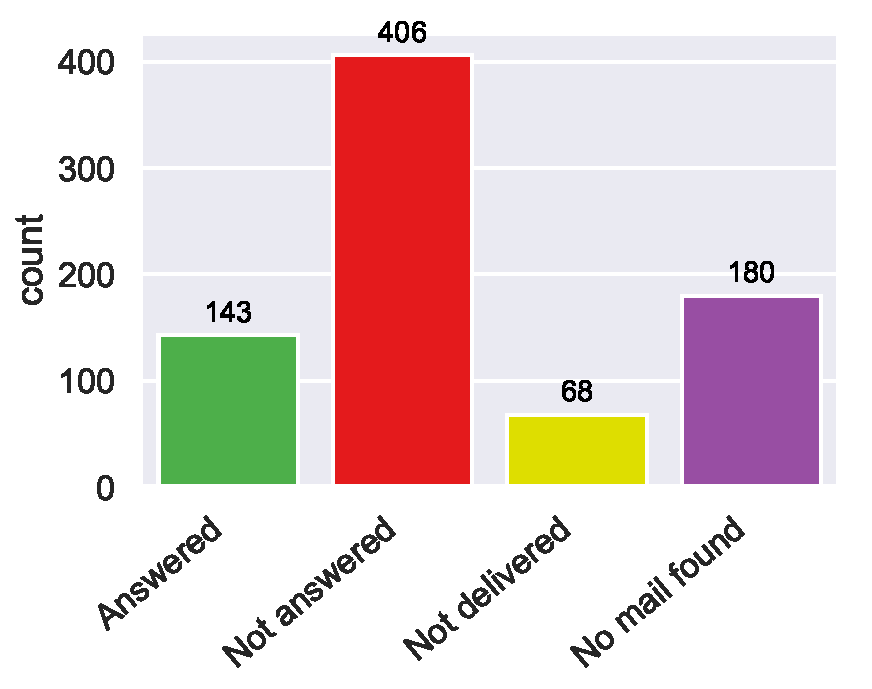
\includegraphics[width=\textwidth, clip]{img/dev-mails/answers-received-builds.pdf}
		\caption{Proportions of logs about which mails were answered, unanswered, not delivered or we could not find a corresponding mail address}
		\label{fig:mails-answers-received-builds}
	\end{minipage}
\end{figure}
\begin{figure}[htbp]
	\centering
	\begin{minipage}{0.45\textwidth}
		\centering
		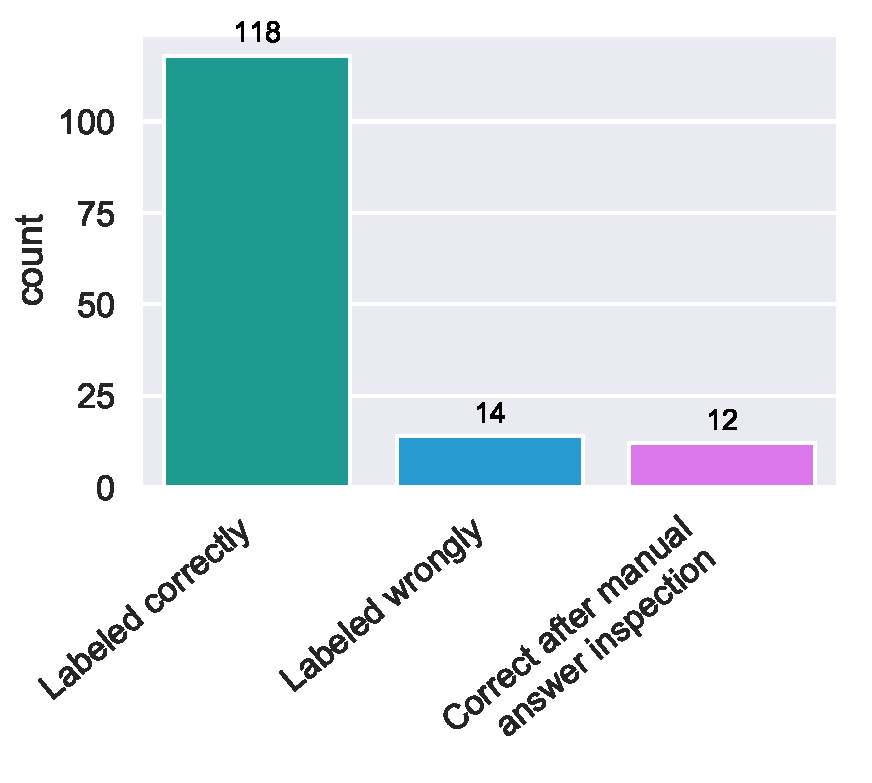
\includegraphics[width=\textwidth, clip]{img/dev-mails/extraction-correct.pdf}
		\caption{Label correctness as validated by developers}
		\label{fig:mails-extraction-correct}
	\end{minipage}\hfill
	\begin{minipage}{0.45\textwidth}
		\centering
		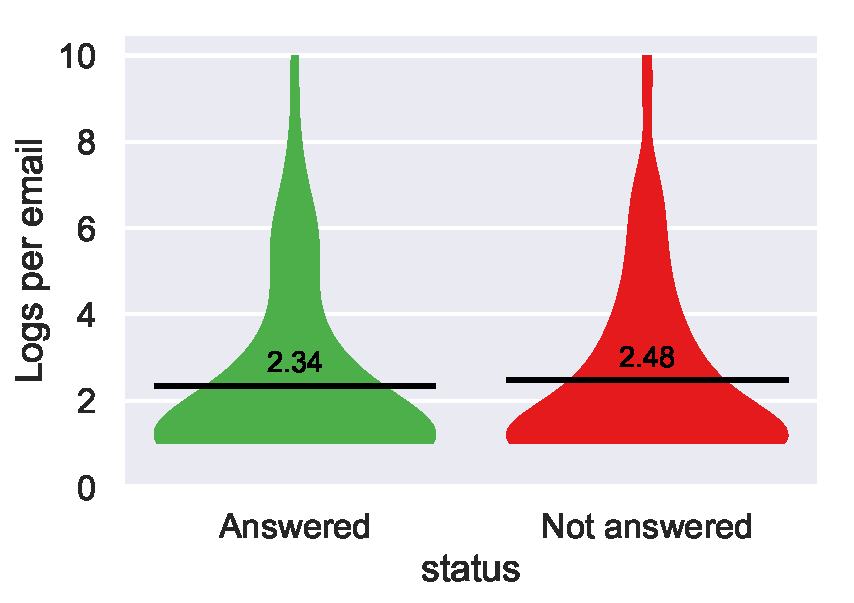
\includegraphics[width=\textwidth, clip]{img/dev-mails/logs-per-mail.pdf}
		\caption{Average number of logs per sent out mail}
		\label{fig:mails-logs-per-mail}
	\end{minipage}
\end{figure}

\paragraph{Results}
In total we sent out mails to 246 developers, asking about 3.2 build logs per mail on average.
32 of these mails could not be delivered, e.g.\ because they were addressed to \emph{noreply} mail addresses.
These 32 mails related to 68 of the build logs.
We received answers from 61 developers, responding about 144 build logs.
Figure~\ref{fig:mails-answers-received-mails} and Figure~\ref{fig:mails-answers-received-builds} show the proportions of mails and logs answered about, not delivered and unanswered.

Of the 144 answers, 132 said our extraction was correct.
26 answered either ``close, but not quite correct'' or ``no, the build failed for another reason''.
We manually inspected these negative answers and found that some extractions were correct after all.
This yields 12 log extractions in our example set that were not correct, shown in Figure~\ref{fig:mails-extraction-correct}.

\paragraph{Discussion}
This study highly strengthens the trust in the validity of the extracted build failure reasons in \emph{LogChunks}.
The study received answers about 18\% of the logs from \emph{LogChunks}.
After manual correction, 91\% of the received answers said our labelled extractions were accurate.

Most of the initial incorrect answers we adjusted in the manual correction, stated that the proposed extraction did not show the whole description of why the build failed.
This is because we had to trim long labeled extractions to keep the mails readable.

One of our extractions only showed a warning and the developer proposed to also include the line above, stating that warnings are treated as errors in the build.
In others that were identified as incorrect, we labelled the error message of an error that later ignored and did not lead to the build failing.

\end{document}
